\chapter{Background and related work}

To adequately contextualize the novel contribution of this thesis, this chapter undertakes a comprehensive review of the existing landscape of software solutions, theoretical frameworks, and academic literature pertinent to vehicle management and sustainable mobility. The primary objective of this chapter is to meticulously map the state of the art, thereby establishing a clear and defensible rationale for the development of the \textit{AlDiaCAR} system. We will systematically examine the current technological offerings across three distinct and highly segmented categories of applications: enterprise-grade commercial fleet management systems, consumer-focused personal car maintenance trackers, and specialized eco-routing navigation tools. This analysis will not only detail the functionalities of existing systems but also critically evaluate their inherent limitations when applied to the specific problem domain of a multi-vehicle, multi-driver household.

\textgap

Furthermore, this review will delve into the theoretical foundations that provide the intellectual scaffolding for this project's design philosophy. Specifically, we will explore the principles of gamification as a mechanism for behavior change and the broader paradigm of Green Information Technology (Green IT), particularly the concept of "Green through IT" or Sustainable Human-Computer Interaction (HCI). By grounding our practical design choices in established academic theory, we aim to enhance the project's robustness and potential for real-world impact. The chapter will culminate in a detailed gap analysis, synthesizing the findings from our market and literature review to precisely identify the unoccupied technological and conceptual niche that the \textit{AlDiaCAR} project is designed to fill. This final section will serve as the definitive justification for the thesis, articulating its unique value proposition and contribution to the field.

\section{State of the art in vehicle management applications}

The contemporary market for vehicle-related software is both mature and extensive, yet it remains conspicuously fragmented. Existing solutions are typically characterized by a high degree of specialization, with software platforms meticulously engineered to target either large-scale commercial enterprises or individual users. This segmentation has resulted in a landscape where tools are powerful within their intended vertical but fundamentally ill-equipped to address the hybrid challenges faced by a modern household managing a small, private fleet of vehicles. The following subsections will dissect each major category, highlighting their capabilities and, more importantly, their shortcomings in relation to the problem statement of this thesis.

\subsection{Commercial fleet management systems}
The Business-to-Business (B2B) sector of fleet management is dominated by powerful, data-intensive software-as-a-service (SaaS) platforms such as \textit{Fleetio} and \textit{Samsara}. These systems are engineered to provide corporations with granular control and comprehensive oversight over large, complex, and geographically dispersed vehicle fleets. Their core value proposition lies in optimizing operational efficiency, ensuring regulatory compliance, and minimizing costs at scale.

\textgap

The feature set of these platforms is consequently vast and sophisticated. Key functionalities typically include:
\begin{itemize}
    \item \textbf{Real-time GPS tracking and geofencing:} Constant monitoring of vehicle location, speed, and heading, coupled with the ability to define virtual perimeters (geofences) that trigger alerts when crossed.
    \item \textbf{Advanced telematics:} Integration with onboard vehicle hardware (often via the OBD-II port) to capture a rich stream of diagnostic data, including engine RPM, fuel consumption, fault codes (DTCs), and harsh braking or acceleration events.
    \item \textbf{Comprehensive maintenance scheduling:} Automated workflows for preventative maintenance based on mileage, engine hours, or calendar intervals, including work order generation and service history logging.
    \item \textbf{Fuel management:} Detailed tracking of fuel purchases, consumption analysis, and integration with fuel card providers to detect fraud or inefficiency.
    \item \textbf{Driver behavior monitoring:} Scoring and reporting on driver performance to identify unsafe or inefficient habits, often used for training and safety programs.
    \item \textbf{Regulatory compliance:} Features designed to automate compliance with regulations such as the Electronic Logging Device (ELD) mandate for hours of service and International Fuel Tax Agreement (IFTA) reporting.
\end{itemize}

\begin{figure}[h!]
    \centering
    \includegraphics[width=0.9\textwidth]{images/background/fleetio.png}
    \caption{Illustrative example of a typical commercial fleet management dashboard (Fleetio), showcasing the complexity and data-density designed for professional logistics managers.}
\end{figure}

\textgap

While these systems represent the pinnacle of vehicle management technology, their direct application to the context of a private household, such as the Martínez family persona, is fundamentally unviable for a confluence of reasons:

\begin{itemize}
    \item \textbf{Prohibitive complexity and cost:} These are enterprise-grade platforms. Their pricing models are typically structured on a per-vehicle, per-month basis, often with substantial setup fees. For a family managing three cars, the cost would be unjustifiable. Moreover, the feature set is overwhelmingly complex, presenting a steep learning curve and a significant cognitive burden for non-technical users.

    \begin{figure}[H]
        \centering
        \includegraphics[width=0.7\textwidth]{images/background/fleetio-pricing.png}
        \caption{Cost of Fleetio starts at 5\$ per vehicle per month if billed monthly, 4\$ if billed annually. Totalling at about 96\$ for a 2 vehicle fleet in the best of the cases.}
    \end{figure}
    
    \textgap
    
    \item \textbf{Misaligned user experience (UX):} The user interface and overall experience are meticulously crafted for a professional fleet manager or dispatcher whose primary job function is to analyze data and manage logistics. The UX prioritizes data density and administrative control over the simplicity, accessibility, and collaborative ease-of-use required for a family context.
    
    \textgap
    
    \item \textbf{Fundamentally different focus:} The teleological purpose of a commercial fleet system is the optimization of business assets to maximize profit and minimize risk. Their design philosophy is rooted in surveillance and control. In contrast, the goal of a personal fleet management tool should be to facilitate collaboration, reduce domestic friction, and promote positive, sustainable habits among trusted users. The underlying motivations are fundamentally different.

    \begin{figure}[H]
        \centering
        \includegraphics[width=0.45\textwidth]{images/background/samsara-mobile.png}
        \caption{Example of a mobile interface for a commercial fleet application (Samsara). The focus remains on asset tracking and driver logs, which is misaligned with the needs of a family.}
    \end{figure}

    \textgap

    \item \textbf{Data privacy and social dynamics:} The level of granular tracking (e.g., real-time location, driving habits) that is standard in a corporate setting is often socially unacceptable and raises significant privacy concerns within a family unit. Implementing such a system could introduce an uncomfortable dynamic of surveillance rather than cooperation.

    \begin{figure}[H]
        \centering
        \includegraphics[width=0.7\textwidth]{images/background/samsara-privacy-issue.png}
        \caption{Every action of the driver is monitored and analysed. In this demo video from Samsara we can see that the driver reaction was stored and analysed}
    \end{figure}

\end{itemize}

\subsection{Personal car maintenance applications}
On the other end of the spectrum are applications developed for the individual car owner. This category includes popular apps like \textit{Drivvo}, \textit{Fuelly}, and \textit{aCar}. These tools are designed to serve as digital logbooks, empowering a single user to meticulously track the health, expenses, and history of their personal vehicle.

\textgap

Their core competency lies in the detailed logging of specific data points. Users can manually record every fuel-up, calculate fuel economy (MPG or L/100km), log all maintenance and repair expenses, and set personalized reminders for crucial service intervals, such as oil changes, tire rotations, or mandatory technical inspections like the Spanish ITV. Many of these applications also offer basic reporting features, allowing users to visualize their spending and fuel consumption over time.

\begin{figure}[H]
    \centering
    \includegraphics[width=0.45\textwidth]{images/background/drivvo-dashboard.png}
    \caption{Typical user interface for a personal car maintenance app like Drivvo, centered on logging fuel, services, and expenses for a single vehicle.}
\end{figure}

\textgap

However, despite their utility for the dedicated single-car enthusiast, their effectiveness rapidly diminishes when applied to the multi-vehicle, multi-driver scenario that this project specifically addresses. Their primary drawbacks include:

\begin{itemize}
    \item \textbf{Inherent single-user, single-vehicle focus:} These applications are architected around the mental model of one person managing one primary vehicle. While some may allow the user to add multiple vehicle profiles, the interface is rarely optimized for comparing them or managing them as a collective "fleet." They lack a centralized dashboard that provides an at-a-glance overview of the entire household's automotive assets.
    
    \textgap
    
    \item \textbf{Absence of collaborative features:} Crucially, these apps are not designed for shared access or collaborative management. They function as data silos on a single user's device. There is no mechanism for multiple family members to view and update the status of a shared vehicle in real-time. This completely fails to address the core problem of "shared maintenance blindness" identified in Chapter 1.
    
    \textgap
    
    \item \textbf{Superficial approach to sustainability:} While fuel economy calculation is a standard feature, its purpose is almost exclusively financial—to help the user track their fuel expenses. These applications do not leverage this data to provide intelligent, forward-looking recommendations. They cannot, for example, advise a user on which of their three cars would be the most ecologically and economically sound choice for an upcoming journey based on its specific parameters.
    
    \textgap
    
    \item \textbf{Passive and utilitarian engagement model:} The vast majority of these apps are functional utilities that require disciplined, manual data entry. They are passive tools that depend entirely on the user's intrinsic motivation. They do not incorporate modern engagement techniques, such as gamification, to actively encourage positive behaviors like performing timely maintenance or adopting more efficient driving habits.
\end{itemize}

\subsection{Eco-routing and navigation tools}
A third category of relevant software has emerged within mainstream navigation applications. In response to growing environmental awareness, technology giants have begun to integrate sustainability-focused features into their platforms. The most prominent example is \textit{Google Maps}, which introduced an "eco-friendly routing" option. This feature's algorithm analyzes various factors, including road incline, traffic congestion, and the number of stops, to suggest a route that is optimized for the lowest possible fuel or energy consumption, often presenting it alongside the fastest route.

\begin{figure}[H]
    \centering
    \includegraphics[width=0.3\textwidth]{images/background/google-maps-ecorouting.png}
    \caption{An illustration of the eco-friendly routing feature in Google Maps.}
\end{figure}

\textgap

While this represents a positive step towards promoting sustainable mobility on a massive scale, the limitation of these tools lies in their profound lack of integration with the user's specific context and available resources. They operate as isolated, single-purpose functions and are consequently incapable of answering the more complex, multi-faceted questions that are central to the problem this thesis addresses. The core deficiencies are:

\begin{itemize}
    \item \textbf{Vehicle agnosticism:} The eco-routing algorithm operates on a generic vehicle model or a very basic user selection (e.g., gasoline, diesel, electric). It is entirely unaware of the specific set of vehicles a user actually owns, their individual efficiencies, their real-time maintenance status, or their regulatory constraints (like a \gls{distintivo-ambiental}).
    
    \textgap
    
    \item \textbf{Inability to recommend a vehicle:} The system can optimize the route for a given, abstract car, but it fundamentally cannot help the user choose the optimal car for that route from their personal fleet. It cannot advise the Martínez family on whether to take the diesel hatchback or the gasoline sedan for a specific trip into the city.
    
    \textgap
    
    \item \textbf{Disconnection from broader management goals:} The feature is transactional and ephemeral. It provides a recommendation for a single journey and is completely disconnected from the user's long-term vehicle management goals, such as managing upcoming maintenance, or tracking a cumulative household carbon footprint.
\end{itemize}

\textgap

The decision-making process for a multi-vehicle household is a complex tree of interdependent variables, which current eco-routing tools are not equipped to navigate. The following diagram illustrates a simplified version of this logic.

\textgap

\begin{figure}[H]
    \centering
    \includegraphics[width=1\textwidth]{images/background/simplified-decision-flow.png}
\end{figure}

\section{Theoretical foundations}

The design and implementation of the \textit{AlDiaCAR} system are not based merely on functional requirements but are deeply informed by established theoretical principles from the fields of human-computer interaction (HCI) and sustainable computing. By leveraging these academic frameworks, the project aims to create a solution that is not only useful but also engaging and genuinely effective at influencing user behavior.

\subsection{Gamification for behavior change}
Gamification is a concept that has gained significant traction in HCI research and practice over the past decade. It is formally defined as "the use of game design elements in non-game contexts" \cite{deterding2011gamification}. The core premise is that the motivational techniques that make games so compelling—such as points, badges, leaderboards, and progress bars—can be extracted and applied to real-world applications to increase user engagement and encourage specific, desirable behaviors.

\textgap

In the context of \textit{AlDiaCAR}, gamification is not a superficial addition but a core mechanic designed to foster long-term habit formation. The application aims to provide positive reinforcement for actions that align with the goals of sustainability and responsible vehicle ownership. For example:
\begin{itemize}
    \item \textbf{Achievements and badges:} Users can earn badges for achievements like "Eco-Warrior" (consistently choosing the lowest-emission vehicle), "Maintenance Master" (logging all service on time), or "Planner Pro" (coordinating vehicle usage ahead of time).
    \item \textbf{Progress statistics:} The application will provide clear, visual feedback on the family's collective progress, showing trends in fuel savings, CO\textsubscript{2} reduction, and money saved. This makes the positive impact of their choices tangible and rewarding.
\end{itemize}

\textgap

This approach is supported by a large body of empirical research. A comprehensive meta-analysis by Hamari et al. concluded that gamification is effective in a variety of domains, with significant positive outcomes for user engagement and behavior change, provided it is thoughtfully implemented and aligned with user motivations \cite{hamari2014does}. The following diagram illustrates the intended motivational loop within \textit{AlDiaCAR}.

\begin{figure}[H]
    \centering
    \includegraphics[width=0.7\textwidth]{images/background/gamification-mermaid.png}
\end{figure}

\subsection{Green IT and sustainable HCI}
This project is fundamentally an exercise in Green Information Technology (Green IT), a field that explores the intersection of computing and environmental sustainability. Green IT is often bifurcated into two distinct sub-domains:
\begin{enumerate}
    \item \textbf{Green in IT:} This focuses on reducing the direct environmental impact of the computing industry itself, through measures like creating energy-efficient data centers, designing recyclable hardware, and reducing e-waste.
    \item \textbf{Green through IT (or ICT for Sustainability):} This focuses on leveraging information and communication technologies (ICT) as a tool to effect positive environmental change in other domains of society. This project is a clear exemplar of this second category.
\end{enumerate}

\textgap

\textit{AlDiaCAR} uses software as a persuasive technology to influence user behavior in the physical world—specifically, their transportation choices—leading to tangible environmental benefits such as reduced fuel consumption and lower greenhouse gas emissions. This approach directly aligns with research by scholars like Berkhout and Hertin, who analyzed the complex role of digital technologies in mediating environmental impacts. They argue that while technology can help to "de-materialise" economic activity (e.g., by replacing physical travel with teleconferencing), it can also lead to "re-materialise" effects or rebounds, where efficiency gains are offset by increased consumption \cite{berkhout2004de}. A well-designed system like \textit{AlDiaCAR} must be conscious of these potential rebounds and focus on promoting a net reduction in environmental impact, not merely more efficient consumption. This project, therefore, contributes to the field of Sustainable HCI by providing a practical case study in designing digital interventions for real-world ecological benefit.

\section{Gap analysis and niche identification}
The comprehensive review of the state of the art in both commercial and personal vehicle management software, as well as the underlying theoretical frameworks, reveals a distinct and underserved gap in the existing technological landscape. While highly specialized tools exist for corporate fleets, individual car enthusiasts, and generic navigation, no current solution holistically integrates their respective functionalities into a single, cohesive platform designed specifically for the collaborative context of a private, multi-vehicle household. This synthesis of capabilities represents the core contribution and unique value proposition of the \textit{AlDiaCAR} project, as illustrated conceptually in Figure \ref{fig:gap-analysis-diagram}.

\begin{figure}[h!]
    \centering
    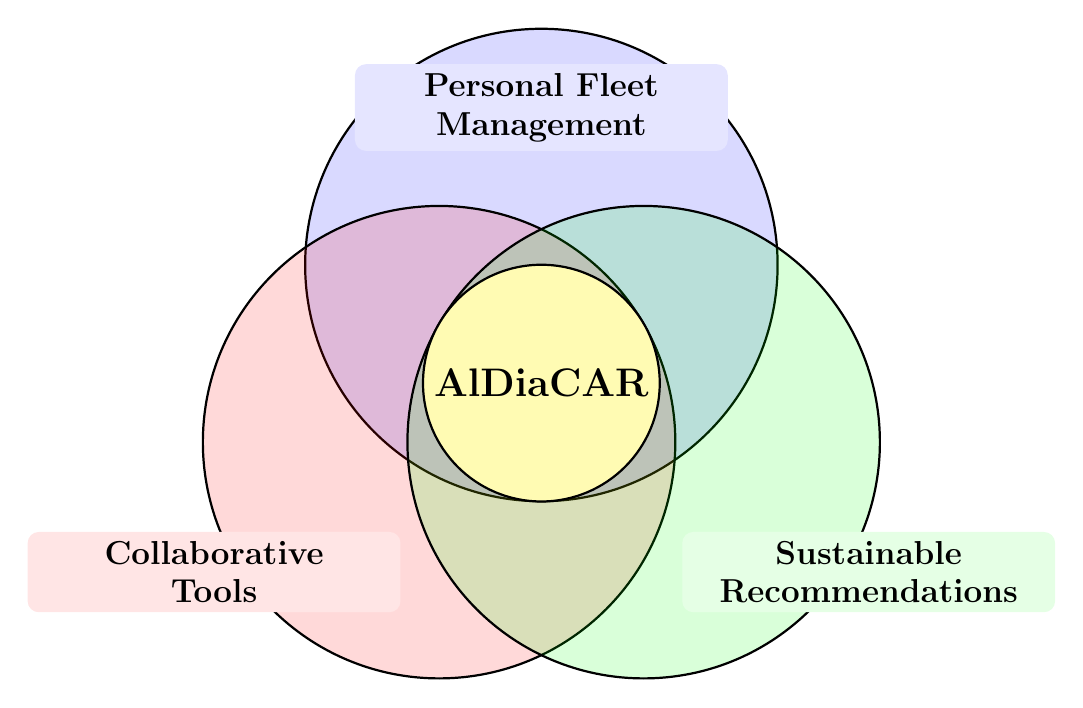
\begin{tikzpicture}[
        % Style for the main circles
        venn-circle/.style={
            draw,
            circle,
            minimum size=6cm,
            fill opacity=0.15,
            text opacity=1,
            thick
        },
        % Style for the main, overarching category labels
        category-label/.style={
            text width=4.5cm,
            align=center,
            font=\bfseries\large
        }
    ]
    
    % Draw the three main circles representing the market domains
    % Positioned at the vertices of an equilateral triangle around the origin
    \node[venn-circle, fill=blue] at (90:1.5cm) {};
    \node[venn-circle, fill=red] at (210:1.5cm) {};
    \node[venn-circle, fill=green] at (330:1.5cm) {};
    
    % Place the main category labels outside the circles, also forming an equilateral triangle
    \node[category-label, rectangle, rounded corners, fill=blue!10] at (90:3.5cm) {Personal Fleet \\ Management};
    \node[category-label, rectangle, rounded corners, fill=red!10] at (210:4.8cm) {Collaborative \\ Tools};
    \node[category-label, rectangle, rounded corners, fill=green!10] at (330:4.8cm) {Sustainable \\ Recommendations};
    
    % Highlight the central intersection, representing the market gap
    \node[font=\bfseries\Large, fill=yellow!30, circle, minimum size=2cm, draw, thick] at (0,0) {AlDiaCAR};

    \end{tikzpicture}
    \caption{Visual representation of the market gap. AlDiaCAR is positioned at the intersection of Personal Fleet Management, Sustainable Recommendations, and Collaborative Tools, a niche not currently occupied by existing solutions.}
    \label{fig:gap-analysis-diagram}
\end{figure}

To further delineate this unoccupied niche, Table \ref{tab:gap_analysis} provides a detailed comparative analysis, summarizing the limitations of existing application categories against the key requirements derived from our problem statement.

\begin{table}[h!]
    \centering
    \caption{Detailed gap analysis of existing application categories}
    \label{tab:gap_analysis}
    \resizebox{\textwidth}{!}{%
    \begin{tabular}{p{0.22\textwidth}|p{0.22\textwidth}|p{0.22\textwidth}|p{0.22\textwidth}|p{0.22\textwidth}}
        \hline
        \textbf{Application category} & \textbf{Target user} & \textbf{Core functionality} & \textbf{Sustainability focus} & \textbf{Identified gaps for AlDiaCAR Project} \\
        \hline
        Commercial Fleet Management Systems & Professional Fleet Manager (B2B) & Logistics, cost control, driver surveillance, large-scale analytics. & Primarily financial (fuel cost reduction); operational efficiency. & Prohibitively expensive and complex for personal use; lacks collaborative, non-surveillance model; misaligned UX and social context. \\
        \hline
        Personal Maintenance Apps & Individual Car Enthusiast (B2C) & Manual logging of fuel, expenses, and service for a single vehicle. & Minimal; limited to calculating fuel economy for financial tracking. & No collaborative features for shared management; poor multi-vehicle comparison; passive, utilitarian engagement model. \\
        \hline
        Eco-Routing \& Navigation Tools & General Driver / Commuter (B2C) & Calculating a fuel-efficient route for a single, generic journey. & High; focused on optimizing a single trip's route for a generic vehicle model. & Disconnected from user's actual vehicle fleet; cannot recommend the optimal vehicle, only the optimal route; lacks maintenance context. \\
        \hline
    \end{tabular}%
    }
\end{table}

\textgap

Therefore, this thesis project, \textit{AlDiaCAR}, is strategically positioned to fill this clearly defined niche. It is conceived as the first mobile application to holistically address the complex needs of an individual or family managing multiple vehicles by uniquely unifying three critical pillars of functionality into a single, user-friendly experience.

\textgap

First, it provides robust \textbf{Personal fleet management} capabilities. This goes beyond the single-vehicle logbook model by offering a centralized, collaborative dashboard where all family members can view the real-time status, location, and maintenance needs of every vehicle in the household fleet. This directly addresses the critical pain point of "shared maintenance blindness" and reduces "coordination friction."

\textgap

Second, the system incorporates \textbf{Integrated sustainability recommendations}. Unlike generic eco-routers, \textit{AlDiaCAR} leverages the detailed data of the user's specific fleet. Its recommendation engine will consider not only the destination but also the unique emissions profile, fuel efficiency, maintenance status, and regulatory constraints of each available vehicle to suggest the holistically optimal car for every journey. This transforms the application from a passive data logger into an active decision-support tool.

\textgap

Third, it implements a thoughtful \textbf{Behavioral reinforcement} layer through gamification. By embedding game-like elements such as badges, progress tracking, and positive feedback, the application aims to make sustainable choices and diligent vehicle care intrinsically rewarding. This actively encourages long-term habit formation, moving beyond mere utility to foster genuine user engagement and a collective household commitment to more sustainable mobility.

\textgap

By seamlessly combining these three pillars, the \textit{AlDiaCAR} project provides a novel and significant contribution to the field of Sustainable HCI. It offers a practical, user-centric tool designed to empower individuals and families to systematically reduce their personal transportation footprint, mitigate household friction, and manage their shared assets more efficiently and responsibly. This chapter has established the clear need and opportunity for such a solution, setting the stage for the subsequent chapters which will detail its design, implementation, and evaluation.
